\documentclass{rapport}
\usepackage{lipsum}
\usepackage{gensymb}
\usepackage{float}
\usepackage{graphicx} % Required for inserting images
\usepackage{amsthm} 
\usepackage{amssymb}
\usepackage{cancel}
\usepackage{polynom}

\usepackage{enumitem}
\usepackage[most, theorems]{tcolorbox}
\usepackage{xcolor}
%\usepackage[italian]{babel} % lingua italiana

%\usepackage[utf8]{inputenc}
\usepackage{pgfplots}
\pgfplotsset{compat=1.18}

\usepackage{tikz}
\usetikzlibrary{calc, angles, quotes}
\newcommand*\circled[2][]{%
  \tikz[baseline=(char.base)]{
    \node[shape=circle,draw=#1,inner sep=1pt] (char) {$\displaystyle #2$};
  }%
}
\usetikzlibrary{patterns}

\usetikzlibrary{arrows.meta}
\usetikzlibrary{matrix, positioning}

\newtcbtheorem{teorema}{Teorema}{
  colback=blue!5!white,
  colframe=blue!75!black,
  enhanced,
  fonttitle=\bfseries,
}{theo}

\newtcbtheorem{definizione}{Definizione}{
    colback=green!5!white, 
    colframe=green!75!black, 
    enhanced,
    fonttitle=\bfseries,
}{def}

\newtcbtheorem{esercizio}{Esercizio}{
    colback=red!5!white, 
    colframe=red!75!black, 
   enhanced,
  fonttitle=\bfseries,
}{es}

\newtcbtheorem{corollario}{Corollario}{
    colback=pink!5!white, 
    colframe=pink!75!black, 
    enhanced,
  fonttitle=\bfseries,
}{corr}

\newtcbtheorem{proposizione}{Proposizione}{
    colback=cyan!5!white, 
    colframe=cyan!75!black, 
    enhanced,
  fonttitle=\bfseries,
}{esem}

% \newtheorem{theorem}{Teorema}
% \newtheorem{proposition}[theorem]{Proposizione}
% \newtheorem{corollary}[theorem]{Corollario}
% \newtheorem{lemma}[theorem]{Lemma}

% \theoremstyle{definition}
% \newtheorem{definition}[theorem]{Definizione}
% \newtheorem{axiom}[theorem]{Assioma}
% \newtheorem{example}[theorem]{Esempio}

% \theoremstyle{remark}
% \newtheorem{remark}[theorem]{Remark}
% \newtheorem{note}[theorem]{Note}
\def\mathunderline#1#2{\color{#1}\underline{{\color{black}#2}}\color{black}}
\newcommand{\mathrect}[2]{%
  \fcolorbox{#1}{white}{\strut$\displaystyle #2$}%
}

\title{DataBase} %title of the file

\begin{document}

%----------- Report information ---------

\logo{logos/logo.jpg}
\uni{\textbf{Università degli Studi di Padova}}
\ttitle{Fisica 2} %title of the file
\subject{Fisica 2} % Subject name
\topic{Fisica 2} % Topic name

\students{Alex Gasparini} % information related to the students

%----------- Init -------------------
        
\buildmargins % display margins
\buildcover % create the front cover of the document
\toc % creates the table of contents

%------------ Report body ----------------



\section{Cariche Elettriche}
\addcontentsline{toc}{subsection}{Le Cariche Elettriche }
Questo corso sarà un viaggio per scoprire come funziona l'elettromagnetismo, che è quella teoria formulata da \textbf{ James Clerk Maxwell} a metà del 1800. Questa teoria riesce a descrivere tutti i fenomeni elettrici e magnetici e le loro interazioni. Pertanto partiamo capendo cos'è l'elettrostatica.

\begin{definizione}{Carica Elettrica}{}
  La \textbf{carica elettrica} è una proprietà intriseca della materia, e può essere \textbf{positiva} o \textbf{negativa}. Le particelle elementari che provocano questa proprietà sono i \textbf{protoni} (per la carica positiva) e gli \textbf{elettroni} per la carica negativa.
\end{definizione}

Quindi la carica elettrica è una caratteristica che ha la materia, proprio come la massa, e infatti vedremo che ci sono molti parallelismi con quest'ultima. La principale differenza tra massa e la carica di un corpo è che la carica può essere sia positiva che negativa, al contrario della massa che può essere solo positiva.

La carica elettrica la indichiamo con la lettera $q$ e unità di misura il \textbf{Coulomb} $[C]$.

\begin{proposizione}{Principio di Quantizzazione della Carica}{}
  La carica di un corpo può essere solamente un multiplo intero della carica fondamentale ($e$) dove 
  \[
  e = 1.6022 \cdot 10^{-19} C
  \]
  Dove l'elettrone avrà carica $q_e = -e$ e il protone $q_p = +e$
\end{proposizione}

Questo perchè da come sappiamo dalla teoria atomica, gli atomi sono indivisibili. Pertanto la carica di un corpo (positiva o negativa che sia) può essere solo un multiplo intero della carica fondamentale. Di conseguenza questo principio ci permette di calcolare il numero di elettroni (o protoni) in un corpo carico elettricamente con la seguente formula 
\[
q = ne
\]

Dove $q$ è la carica del corpo, $n$ è il numero di particelle e $e$ la carica fondamentale. 

Dato che prima abbimo parlato di massa è interessante vedere la relazione tra la massa dell'eletrrone e del protone

\begin{table}[!h]
  \centering
\begin{tabular}{l|l|l}
          & Carica Elettrica                                           & Massa          \\ \hline
Protone   & $+1.6022 \cdot 10^{-19} C$ & $1.6726 \cdot 10^{-27} kg$ \\ \hline
Elettrone & $-1.6022 \cdot 10^{-19} C$ & $9.1094 \cdot 10^{-31} kg$
\end{tabular}
\end{table}



Interessante è notare come la carica elettrica sia identica a parte per il segno, mentre la massa sia completamente diversa, infatti il protone è più grande di 4 ordini di grandezza. 



\newpage

\begin{proposizione}{Principio di Conservazione della Carica}{}
  In un sistema isoltato, la somma delle cariche elettriche del sistema resta sempre costante.
\end{proposizione}

Questa è una diretta conseguenza dei principi della teoria atomica, ovvero che i protoni ed elettroni non si creano e non si distruggono, pertanto in un sistema isoltato le cariche di un sistema saranno sempre quelle, al massimo si potranno spostare ma non possono scomparire o apparire.

\begin{definizione}{Forza di Coulomb}{}
  Due cariche nello spazio $q_1, q_2$ sono sottoposte ad una forza, detta di Coulomb,  pari  
  \[
  \vec{F}_{12} = \dfrac{1}{4\pi \varepsilon_0} \dfrac{q_1q_2}{d^2} \hat{u}_{12}
  \]

  Dove $\vec{F}_{12}$ è la forza esercitata da $q_1$ sulla carica $q_2$, $\varepsilon_0$ è la costante dielettrica nel vuoto, e vale 
  \[\varepsilon_0=8.85\cdot 10^{-12} \dfrac{C^2}{Nm^2}\]
  $d$ è la distanza tra le due cariche e $\hat{u}_{12}$ è il versore che parte da $q_1$ e punta $q_2$.
\end{definizione}


La forza di Coulomb è molto simile di struttura a quella gravitazionale, l'unica cosa che cambia è che al posto delle masse abbiamo le cariche elettriche e cambia la costante moltiplicativa. Ricordiamo che le cariche possono essere negative, quindi se prendiamo $q_1q_2<0$ allora la forza sarà attrattiva, altrimenti la forza è repulsiva.

\begin{esercizio}{}{}
Calcolare il rapporto tra forza di Coulomb e la forza gravitazionale  in un atomo di idrogeno, evvero di un elettrone e di un protone distanti $d=5.29\cdot 10^{-11}m$. 
\end{esercizio}

\begin{proof}[svolgimento]
  Per questo esercizio c'è solo da mettere dentro i numeri e ricordarsi la formula della forza gravitazionale. I valori della carica elettrica e massa di protone ed elettorne sono scritte sulla tabella a pagina precedente

  \[
  ||\vec{F}_c|| = \dfrac{1}{4\pi\varepsilon_0} \dfrac{q_e \cdot q_p }{d^2} = \dfrac{1}{4\pi \cdot 8.85\cdot 10^{-12}} \dfrac{|-1.6\cdot 10^{-19} \cdot +1.6\cdot 10^{-19}|   }{(5.29\cdot 10^{-11})^2} \approx 8.23 \cdot 10^{-8} N
  \]


  \[
  ||\vec{F}_g|| = G \dfrac{m_e \cdot m_p }{d^2} = 6.67\cdot 10^{-11}  \dfrac{1.67\cdot 10^{-27} \cdot 9.1\cdot 10^{-31}   }{(5.29\cdot 10^{-11})^2} \approx 3.62 \cdot 10^{-47} N
  \]


  \[
  \dfrac{||F_c||}{||F_g||} = \dfrac{8.23 \cdot 10^{-8} N }{3.62 \cdot 10^{-47} N} \approx 2.27 \cdot 10^{39}
  \]
\end{proof}

Da questo semplice esercizio possiamo notare come a livello microscopico la forza di Coulomb è nottamente più predominate di quella gravitazionale, infatti quella gravitazionale è circa $10^{40}$ volte più grande.

\newpage

\begin{proposizione}{Principio di Sovvraposizione degli Effetti}{}
  Siano $n$ corpi carichi elettricamente con carica $q_i$, allora la forza di Coulomb risultate su un corpo $j$ è la somma vettoriale delle forze con tutti gli altri corpi
  \[
  \vec{F}^{tot}_j = \sum_{i\ne j} \vec{F}_{ij}
  \]
\end{proposizione}

L'idea è molto semplice è anche molto intuitiva di questo concetto, infatti è identico a quello che avevamo visto con la forza gravitazionale, quindi vediamo subito un esercizio 

\begin{esercizio}{}{}
  Siano 3  elettroni posti ai vertici di un triangolo equilatero di lato $l$. Scrivere la forze che subiscono i tre elettroni. 
\end{esercizio}

\begin{proof}[svolgimento]
  Come tutti i problemi di fisica, facciamoci un disegno esplicativo
\begin{center}
  

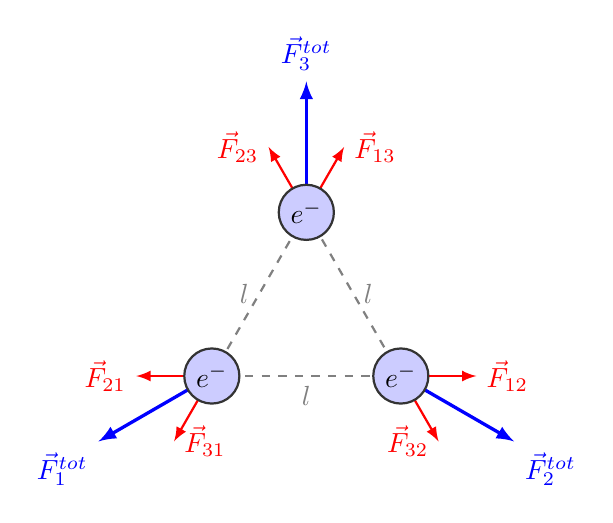
\begin{tikzpicture}[
    scale=0.8,
    charge/.style={circle, draw=black!80, fill=blue!20, thick, inner sep=2pt, minimum size=7mm},
    force/.style={->, >=latex, red, thick},
    resultant/.style={->, >=latex, blue, very thick}
]

    % Definisco la lunghezza del lato per il disegno (l)
    \def\a{3} 
    % Definisco la lunghezza dei vettori forza
    \def\f{1.2} 

    % Coordinate dei vertici del triangolo equilatero
    \coordinate (q1) at (0,0);
    \coordinate (q2) at (\a,0);
    \coordinate (q3) at (\a/2,{\a*sqrt(3)/2});

    % 1. Disegno i lati del triangolo
    \draw[dashed, thick, gray] (q1) -- (q2) node[midway, below] {$l$};
    \draw[dashed, thick, gray] (q2) -- (q3) node[midway, right] {$l$};
    \draw[dashed, thick, gray] (q3) -- (q1) node[midway, left] {$l$};

    % 2. Disegno i vettori forza (disegnati prima così "escono" dal bordo delle cariche)
    
    % Forze sull'elettrone 3 (vertice in alto)
    \draw[force] (q3) -- ++(60:\f) node[right] {$\vec{F}_{13}$};
    \draw[force] (q3) -- ++(120:\f) node[left] {$\vec{F}_{23}$};
    \draw[resultant] (q3) -- ++(90:{\f*sqrt(3)}) node[above] {$\vec{F}^{tot}_{3}$};

    % Forze sull'elettrone 1 (vertice in basso a sinistra)
    \draw[force] (q1) -- ++(240:\f) node[right] {$\vec{F}_{31}$};
    \draw[force] (q1) -- ++(180:\f) node[left] {$\vec{F}_{21}$};
    \draw[resultant] (q1) -- ++(210:{\f*sqrt(3)}) node[below left] {$\vec{F}^{tot}_{1}$};

    % Forze sull'elettrone 2 (vertice in basso a destra)
    \draw[force] (q2) -- ++(300:\f) node[left] {$\vec{F}_{32}$};
    \draw[force] (q2) -- ++(360:\f) node[right] {$\vec{F}_{12}$};
    \draw[resultant] (q2) -- ++(330:{\f*sqrt(3)}) node[below right] {$\vec{F}^{tot}_{2}$};

    % 3. Disegno le cariche (nodi) sopra i vettori
    \node[charge] at (q1) {$e^-$};
    \node[charge] at (q2) {$e^-$};
    \node[charge] at (q3) {$e^-$};

\end{tikzpicture}
\end{center}


Per simmetria del triangolo è facile intuire che gli elttroni avranno tutti la stessa forza complessiva $||\vec{F}^{tot}_{1}|| = ||\vec{F}^{tot}_{2}|| = ||\vec{F}^{tot}_{3}||$, quindi basta che ci focaliziamo su una soltanto, quindi prendiamo il vertice superiore come riferimento. Quindi per il principio di sovvraposizione sappiamo che
\[
\vec{F}^{tot}_{3} = \vec{F}_{23} + \vec{F}_{13}
\]
Quindi procediamo a calcolare le forze, che sempre per simmetria vale $||\vec{F}_{23}||=||\vec{F}_{13}||$
\[
||F_{i3}|| = \dfrac{1}{4\pi \varepsilon_0} \dfrac{q_e^2}{l^2} = \dfrac{1}{4\pi \cdot 8.85\cdot 10^{-12}} \dfrac{(-1.6\cdot 10^{-19})^2   }{l^2} \approx  \dfrac{2.3\cdot 10^{-28}}{l^2}
\]

Ora pero dobbiamo ricordarci che è la somma vettoriale, quindi con un po' di geometria riconosciamo che 
\[
||\vec{F}^{tot}_3|| = 2||\vec{F}_{i3}||\cos\dfrac{\pi}{6} = 2 \cdot \dfrac{2.3\cdot 10^{-28}}{l^2} \cdot \dfrac{\sqrt{3}}{2} \approx \dfrac{3.98\cdot 10^{-28}}{l^2}
\]
\end{proof}


\newpage
\begin{definizione}{Campo Elettrico}{}
  Sia una carica elettrica $q_1$ nello spazio, allora possiamo definire una nuova funzione \textbf{campo elettrico} come 
  \[
  \vec{E}(d) = \lim_{q_0\to 0} \dfrac{\vec{F}_{10}}{q_0}
  \]
  Dove $q_0$ è una carica generica e $\vec{F}_{10}$ è la forze di Coulomb subita da $q_0$
\end{definizione}

Possiamo sviluppare la definizione usando la formula della forza di Coulomb


\[
  \vec{E}(d) =  \lim_{q_0\to 0} \dfrac{1}{q_0} \dfrac{1}{4\pi\varepsilon_0} \dfrac{q_1 q_0}{d^2}\hat{u}_{10} = \dfrac{1}{4\pi\varepsilon_0} \dfrac{q_1}{d^2} \hat{u}_{10}
\]


Che in forma differenziale diventa

\[
dE = \dfrac{1}{4\pi\varepsilon_0} \dfrac{dq}{d^2} \hat{u} 
\]

Poi dato che il campo elettrico non è altro che un modo per normalizzare la forza indipendentemente dalla forza, rispetta il principio di sovvraposizione degli effetti, quindi il ragionamento che abbiamo fatto per l'esercizio del tringolo lo possiamo applicare anche al campo elettrico.

Per ora pensiamo al campo elettrico come una funzione che definiamo noi per semplificarci i conti, quindi per ora per noi è solo uno strumento matematico che vedremo che ci aiuterà molto. Verso la fine del corso vedremo che in realtà il campo elettrico è un qualcosa di vero e prorpio fisicamente, non è solo uno strumento matematico, ma questo lo vedremo con le equazioni di Maxwell.

\begin{definizione}{Distribuzione di Carica}{}
  Le cariche di un corpo possono essere descritte da una funzione \textbf{distribuzione di carica}, che definiamo 
  \begin{itemize}
    \item \textbf{Lineare} (monodimensionale) definita come 
    $dq = \lambda dx$
    \item \textbf{Superficiale} (bidimensionale) definita come 
    $dq = \sigma d\Sigma$
     \item \textbf{Volumetrica} (tridimensionale) definita come 
   $ dq = \rho dxdydz$
  \end{itemize}
\end{definizione}

L'idea dietro alla distribuzione di carica è che se noi abbiamo una carica con tante particelle fondamentali, allora noi possiamo approssimarla ad una distribuzione uniforme descritta dalla relativa funzione ($\lambda$,$\sigma$,$\rho$) in modo tale che la distribuzione sembra una funzione continua e non una discretizzazione dovuta alla quantizzazione delle particelle fondamentali.

Questo lo possiamo fare proprio perchè per nelle applicazioni di tutti i giorni difficilmente usiamo poche cariche, ad esempio anche se non abbiamo ancora visto il concetto di corrente, se in un filo passa $1A$ di corrente vuol dire che stanno passando circa $10^{19}$ particelle ogni secondo, il che ci permette di rendere continua la distribuzione perchè si avvicina molto alla realtà.


\begin{esercizio}{}{}
  Sia un filo infinitamente lungo con densità di carica lineare costante $\lambda$, trovare la funzione campo elettrico in funzione della distanza $r$ dalla retta.
\end{esercizio}

\begin{proof}[svolgimento]
  Per capire bene questo problema è fondamentale fare un disegno fatto per bene. Iniziamo scegliendo l'asse x per rappresentare il filo infinito. Poi per comodità il punto distante $r$ lo poniamo sull'asse y. Ora prendiamo una qualsiasi carica $dq$ sull'asse x, e troviamo la distanza tra $dq$ e il punto $(0, r)$ (che è il punto dove vogliamo trovare il campo elettrico)

  \begin{center}
    
  \begin{tikzpicture}[
    scale=0.8,
    >=latex,
    vector/.style={->, thick, red},
    component/.style={->, dashed, red!80},
    wire/.style={very thick, blue}
]

    % Assi cartesiani
    \draw[->, gray] (-5.5, 0) -- (5.5, 0) coordinate (X_axis) node[right, black] {$x$};
    \draw[->, gray] (0, -1) -- (0, 3.5) coordinate (Y_axis) node[above, black] {$y$};
    \coordinate (O) at (0,0);

    % Filo infinito (asse x)
    \draw[wire] (-4.5, 0) -- (4.5, 0) ;
    \draw[wire, dashed] (4.5, 0) -- (5, 0);
    \draw[wire, dashed] (-4.5, 0) -- (-5, 0);

    % Punto P sull'asse y
    \def\r{2.5}
    \coordinate (P) at (0, \r);
    \fill (P) circle (1.5pt) ;
    \coordinate (P_up) at (0, \r+2); % Punto ausiliario per l'angolo

    % Quota r (distanza del punto dal filo)
    \draw[<->] (-0.3, 0) -- (-0.3, \r) node[midway, left] {$r$};

    % Elemento di carica dq
    \def\x{3} % coordinata x di dq
    \coordinate (dq) at (\x, 0);
    \draw[line width=4pt, red] (\x-0.2, 0) -- (\x+0.2, 0) node[below=2.5pt, black] {$dq$};
    \draw[<->] (0, -0.3) -- (\x, -0.3) node[midway, below] {$x$};

    % Distanza tra dq e P
    \draw[dashed, thick] (dq) -- (P) node[midway, above right, xshift=-2pt] {$d = \sqrt{r^2 + x^2}$};


    % -------------------------------------------------------------------

\end{tikzpicture}
\end{center}

Ora dal disegno sappiamo che $d=\sqrt{r^2+x^2}$ e mentre dalla definizione di distribuzione di carica sappiamo che $dq = \lambda dx$, da cui possiamo riscrivere la forma differenziale del campo elettrico come 
\[
dE = \dfrac{1}{4\pi\varepsilon_0} \dfrac{\lambda dx}{(\sqrt{r^2+x^2})^2} \hat{u}
\]

$\hat{u}$ è il versore che parte da $dq$ e punta a $(0, r)$, quindi il vettore è $(-x, r)$ da normalizzare che quindi diventa 

\begin{align*}
dE &= \dfrac{1}{4\pi\varepsilon_0} \dfrac{\lambda dx}{(\sqrt{r^2+x^2})^2} \dfrac{1}{\sqrt{x^2+r^2}} \begin{pmatrix}
  -x \\
  r
\end{pmatrix} \\[0.1cm]
&= \dfrac{1}{4\pi\varepsilon_0} \dfrac{\lambda dx}{(r^2+x^2)^{3/2}}\begin{pmatrix}
  -x \\
  r
\end{pmatrix}
\end{align*}

Ora che è tutto apposto possiamo intergrare ambo i membri, e integriamo su tutto $\mathbb{R}$ dato che il filo è infinitamente lungo.

\begin{align*}
\int dE &= \int_{-\infty}^{+\infty}\dfrac{1}{4\pi\varepsilon_0} \dfrac{\lambda dx}{(\sqrt{r^2+x^2})^2} \dfrac{1}{\sqrt{x^2+r^2}} \begin{pmatrix}
  -x \\
  r
\end{pmatrix} \\[0.1cm]
\vec{E}(r) &= \dfrac{\lambda}{4\pi\varepsilon_0} \left[\begin{pmatrix}
  1 \\
  0
\end{pmatrix}\int_{-\infty}^{+\infty}  \dfrac{-x dx}{(r^2+x^2)^{3/2}} + \begin{pmatrix}
  0 \\
  1
\end{pmatrix}\int_{-\infty}^{+\infty}  \dfrac{r dx}{(r^2+x^2)^{3/2}}\right]
\end{align*}


Il primo integrale notiamo che è una funzione dispari su un intervallo simmetrico, quindi sappiamo già che fa 0. Il secondo integrale lo risolviamo con una sostituzione, ponendo $x=r\tan \theta$ così gli estremi diventano $\pm\pi/2$. Poi per semplicità scriviamo il versore $(0, 1)$ come $\hat{y}$

\begin{align*}
  \vec{E}(r) &= \dfrac{\lambda r }{4\pi\varepsilon_0} \hat{y} \int_{-\pi/2}^{\pi/2}\dfrac{r}{(r^2+r^2\tan^2\theta )^{3/2}} \dfrac{d\theta}{\cos^2 \theta} \\
 &= \dfrac{\lambda r^2 }{4\pi\varepsilon_0} \hat{y}  \int_{-\pi/2}^{\pi/2}\dfrac{1}{r^3 \frac{1}{\cos^3\theta}} \dfrac{d\theta}{\cos^2 \theta} \\
 &= \dfrac{\lambda  }{4\pi\varepsilon_0 r} \hat{y}  \int_{-\pi/2}^{\pi/2}\cos\theta d\theta \\
 &= \dfrac{\lambda  }{4\pi\varepsilon_0 r} \hat{y} \left[\sin\left(\dfrac{\pi}{2}\right)-\sin\left(\dfrac{-\pi}{2}\right)\right] \\
 &= \dfrac{\lambda  }{2\pi\varepsilon_0 r} \hat{y} 
\end{align*}
\end{proof}


\end{document}

